\chapter{Results}\label{chap:results}
\section{Convergence Test}
\begin{table}[htb]
  \centering
\caption{Numerical order of convergence of ADER-DG method}%
\label{tab:convergence-order}
\begin{tabular}{@{}lS[table-format=1.2]S[table-format=1.2]S[table-format=1.2]@{}}
\toprule
{Order} & {$L_1$} & {$L_2$} & {$L_\infty$}\\ \midrule
1 & 2.03 & 2.00 & 1.92\\
2 & 2.56 & 2.55 & 2.55\\
3 & 3.43 & 3.40 & 3.44\\
4 & 4.27 & 4.27 & 4.36\\
5 & 5.00 & 5.02 & 5.08\\
6 & 4.46 & 4.50 & 4.65\\
\bottomrule
\end{tabular}
\end{table}

\begin{figure}[htb]
  \centering
  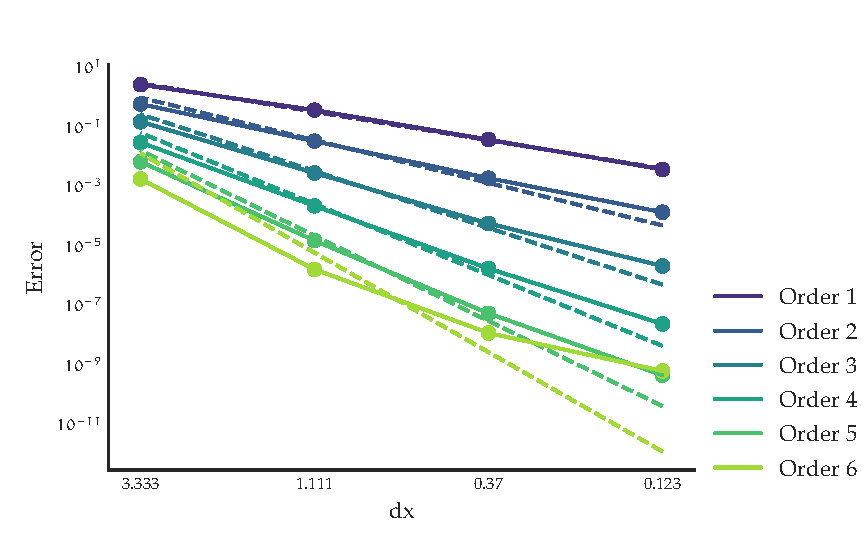
\includegraphics[trim=0.2cm 0.3cm 0.2cm 1.0cm, clip]{thesis_convergence}
  \caption{$L_2$-Error vs.\ Grid Size.
    The dashed lines are the optimal order of convergence $N+1$.
  The line is estimated by using the constant part of a linear regression fit and the ideal order as slope.}
  \label{fig:convergence-l2-error}
\end{figure}

\newcommand{\error}{\operatorname{Total-Error}}

Before computing the error we first need to define the $L_p$ norms for a $p > 0$ by
% notation: https://en.wikipedia.org/wiki/Lp_space#Lp_spaces
\begin{equation}
  \label{eq:Lp-nrom}
  \Vert f(x) \Vert_p = \left( \int_K \vert f(x) \vert^p d\mu  \right)^{1/p}.
\end{equation}
We are interested in the total error which we define as the norm of the difference between an analytical solution $f(\bm{x}, t)$ and our approximation $\hat{f}(\bm{x}, t)$.
The error at a time $t$ is thus defined as
\begin{equation}
  \label{eq:error}
  \error(t,p) = \Vert f(\bm{x}, t) - \hat{f}(\bm{x}, t) \Vert_p.
\end{equation}

We first observe that for our approximation space $\broken$ we can split up the error as a sum over all cells
\begin{equation}
  \label{eq:lp-norm-broken}
 %\Vert f(\bm{x}) \Vert = \sum_{\cell[] \in \broken} \Vert f_{\cell[]} (\bm{x}) \Vert_p,
  \error(t,p) = \sum_{\cell[] \in \broken} \error_{\cell[]}(t,p)
\end{equation}
where $\error_{\cell[]}$ is the error in the cell $\cell[]$.

\todo{Describe how to integrate the error for cells, and effect of volume}
We evaluate the cell-wise error with Gaussian quadrature using \cref{eq:integration-by-substitution}
 \begin{equation}
   \Vert f_K(x) \Vert_p = \left( V \sum_{\bm{i}} \vert f(\bm{x}_i, t) - \hat{f}(\bm{x}_i, t) \vert^p w_{{\bm{i}}}  \right)^{1/p},
 \end{equation}
where $V = \Delta x \Delta y$ is the volume of each two-dimensional cell.
\todo{Use quadNodes, quadWeights and volume macro}
The sum runs over all quadrature nodes $x_i$ with weights $w_i$.
We use ten nodes for all orders and evaluate our solution for all nodes.
In this way we ensure a fair comparision.

For the limiting case of $p \to \infty$ we use the maximum point-wise error.


We compute the error for the manufactured-solution scenario (\cref{sec:manufactured-solution}).
Looking at the plot for the $L_2$ error (refer to plot here) shows that our method converges for all tested polynomial orders.
\todo{Preliminary results used here!}

To compute the numerical order of convergence, we perform a linear regression of the logarithm of the error vs.\ the logarithm of the meshsize.
The size of the slope is then the convergence order.
We can see (\cref{tab:convergence-order}) that our numerical convergence rate increases with the polynomial order.
We do not achieve the optimal theoretical order of convergence of $N+1$.
In~\cite{dumbser2010arbitrary}, which use a similar numerical method and the same scenario, but a different grid, \citeauthor{dumbser2010arbitrary} achieves the optimal order for most polynomial orders.
Some \textsc{dg}-methods of odd order only achieve a numerical convergence order of $N+\nicefrac{1}{2}$.

\section{Accurate CFD}
Show:
\begin{itemize}
\item Taylor-Green High Order
\item ABC Medium Order
\end{itemize}
\section{Accurate Clouds}
\begin{itemize}
\item Cosine Bubble
\item Two Bubbles
\end{itemize}
\section{Time-to-solution: AMR vs Static Mesh}
To show the effectiveness of the \amr{}, we compare the time to solution of a simulation using \amr{} and another simulation with a fully refined mesh.
In detail, we compare
\begin{description}
\item[AMR] We use a coarse mesh with just $9 \times 9$ cells.
  Each cell can be refined up to three times.
  That is, the cells have sidelengths of roughly $\left( \SI{111.1}{\m}, \SI{37.04}{\m}, \SI{12.35}{\m} \right)$.
  As refinement thresholds we use $T_\text{refine} = 2.5$ and $T_\text{delete} = -0.5$ in \cref{eq:refinement-criterion}.
\item[Fine] We use a uniform grid where all cells have a sidelength corresponding to the finest mesh of the \amr{}-test case.
  In addition, we disable the reduction of global observables.
\end{description}
We use an \aderdg{}-method of order $4$ and thus have a minimal effective resolution of ca.\ $\SI{3.09}{\m}$.

To ensure a fair comparison, we ran both configurations with the same optimisation option.

We use a single node of the Haswell-nodes of the Supermuc (Phase 2).
The node has two xxx\todo{name cpus} \textsc{cpu}s with 28 cores each.
Both \textsc{cpu}s currently run on $\SI{1.8}{\GHz}$.
We use the \tbb{} parallelisation of \exahype{}.
To find a reasonable parameter for the number of background threads, we ran a grid search.
We ran three \amr{} testcases for a simulation time of $\SI{1}{\min}$.
\todo{Noisy, show results}
The best median performance was achieved by using six background threads.

Both methods show similar results.
The \amr{}-method took \SI{98654.1}{\s} (\SI{1}{\day} \SI{3}{\hour} \SI{24}{\minute} \SI{14}{\s})
while the fully refined grid took \SI{169071}{\s} (\SI{1}{\day} \SI{22}{\hour} \SI{57}{\minute} \SI{51}{\s}).

no \amr{}:
\begin{verbatim}
 169071       info         memoryUsage    =1390 MB
 169071       info         number of mesh refinements      = 0
 169071       info         number of local recomputations  = 0
 169071       info         number of predictor reruns      = 1
 169071       info         || adapter name       || iterations   || total CPU time [t]=s         || average CPU time/g
rid sweep [t]=s    || total real time [t]=s        || average real time/grid sweep [t]=s  || CPU time properties  || r
eal time properties 
 169071       info         | MeshRefinement      |  5    |  12.58        |  2.516        |  0.593972     |  0.118794 
    |  (2.516,#5,eps=0,max=10.48(value #1),min=0.05(value #0),+316.534%,-98.0127%,std-deviation=3.98956) [not a valid 
averaged value yet]   |  (0.118794,#5,eps=0,max=0.420273(value #1),min=0.0371888(value #3),+253.782%,-68.6948%,std-dev
iation=0.150842) [not a valid averaged value yet]
 169071       info         | FinaliseMeshRefinement      |  1    |  0.52         |  0.52         |  0.0232477    |  0.
0232477    |  (0.52,#1,eps=0,max=0.52(value #0),min=0.52(value #0),+0%,-0%,std-deviation=3.27826e-09) [not a valid ave
raged value yet]     |  (0.0232477,#1,eps=0,max=0.0232477(value #0),min=0.0232477(value #0),+0%,-0%,std-deviation=1.82
031e-10) [not a valid averaged value yet]
 169071       info         | InitialPrediction   |  2    |  0.68         |  0.34         |  0.0334988    |  0.0167494 
   |  (0.34,#2,eps=0,max=0.53(value #0),min=0.15(value #1),+55.8824%,-55.8824%,std-deviation=0.19) [not a valid averag
ed value yet]        |  (0.0167494,#2,eps=0,max=0.0236651(value #0),min=0.0098337(value #1),+41.2893%,-41.2893%,std-de
viation=0.00691571) [not a valid averaged value yet]
 169071       info         | FusedTimeStep       |  1428594      |  4.50835e+06          |  3.15579      |  168823 
      |  0.118174     |  (3.15579,#1.42859e+06,eps=0,max=9.74(value #1409698),min=0.25(value #1119695),+208.639%,-92.0
781%,std-deviation=2.72931) [not a valid averaged value yet]    |  (0.118174,#1.42859e+06,eps=0,max=0.590513(value #12
19442),min=0.011952(value #584763),+399.697%,-89.8861%,std-deviation=0.099553) [not a valid averaged value yet]
 169071       info         | PredictionRerun     |  2    |  7.49         |  3.745        |  0.271615     |  0.135807 
    |  (3.745,#2,eps=0,max=7.07(value #0),min=0.42(value #1),+88.785%,-88.785%,std-deviation=3.325) [not a valid avera
ged value yet]        |  (0.135807,#2,eps=0,max=0.257506(value #0),min=0.0141086(value #1),+89.6113%,-89.6113%,std-dev
iation=0.121699) [not a valid averaged value yet]
 169071       info         | BroadcastAndDropNeighbourMessages   |  1    |  5.92         |  5.92         |  0.216065 
    |  0.216065     |  (5.92,#1,eps=0,max=5.92(value #0),min=5.92(value #0),+0%,-0%,std-deviation=2.67624e-08) [not a 
valid averaged value yet]     |  (0.216065,#1,eps=0,max=0.216065(value #0),min=0.216065(value #0),+0%,-0%,std-deviatio
n=9.81246e-10) [not a valid averaged value yet]
\end{verbatim}

\amr{}:
\begin{verbatim}
98654.1      info         memoryUsage    =1543 MB
 98654.2      info         number of mesh refinements      = 368
 98654.2      info         number of local recomputations  = 0
 98654.2      info         number of predictor reruns      = 151
 98654.2      info         || adapter name       || iterations   || total CPU time [t]=s         || average CPU time/g
rid sweep [t]=s    || total real time [t]=s        || average real time/grid sweep [t]=s  || CPU time properties  || r
eal time properties 
 98654.2      info         | MeshRefinement      |  5411         |  6546.45      |  1.20984      |  259.067      |  0.
0478779    |  (1.20984,#5411,eps=0,max=2.1(value #5358),min=0.01(value #0),+73.5765%,-99.1734%,std-deviation=0.219178)
 [not a valid averaged value yet]    |  (0.0478779,#5411,eps=0,max=0.0876097(value #3782),min=0.00762901(value #5),+82
.9857%,-84.0657%,std-deviation=0.00892198) [not a valid averaged value yet]
 98654.2      info         | FinaliseMeshRefinement      |  1    |  0.13         |  0.13         |  0.00693282   |  0.
00693282   |  (0.13,#1,eps=0,max=0.13(value #0),min=0.13(value #0),+0%,-0%,std-deviation=0) [not a valid averaged valu
e yet]       |  (0.00693282,#1,eps=0,max=0.00693282(value #0),min=0.00693282(value #0),+0%,-0%,std-deviation=0) [not a
 valid averaged value yet]
 98654.2      info         | FinaliseMeshRefinementOrLocalRollback       |  368          |  461.67       |  1.25454 
     |  18.1743      |  0.0493866    |  (1.25454,#368,eps=0,max=1.83(value #341),min=0.67(value #0),+45.8704%,-46.5939
%,std-deviation=0.171853) [not a valid averaged value yet]     |  (0.0493866,#368,eps=0,max=0.0706977(value #356),min=
0.0267934(value #0),+43.1517%,-45.7475%,std-deviation=0.00629674) [not a valid averaged value yet]
 98654.2      info         | InitialPrediction   |  2    |  0.13         |  0.065        |  0.00881638   |  0.00440819
   |  (0.065,#2,eps=0,max=0.07(value #0),min=0.06(value #1),+7.69231%,-7.69231%,std-deviation=0.005) [not a valid aver
aged value yet]      |  (0.00440819,#2,eps=0,max=0.00483773(value #0),min=0.00397865(value #1),+9.74412%,-9.74412%,std
-deviation=0.00042954) [not a valid averaged value yet]
 98654.2      info         | FusedTimeStep       |  1427510      |  2.54517e+06          |  1.78294      |  98033.6 
     |  0.0686745    |  (1.78294,#1.42751e+06,eps=0,max=5.73(value #1227908),min=0.12(value #1),+221.379%,-93.2696%,st
d-deviation=1.05159) [not a valid averaged value yet]          |  (0.0686745,#1.42751e+06,eps=0,max=0.43664(value #141
3800),min=0.00461528(value #1),+535.811%,-93.2795%,std-deviation=0.0435888) [not a valid averaged value yet]
 98654.2      info         | PredictionRerun     |  302          |  403.06       |  1.33464      |  14.4881      |  0.
0479739    |  (1.33464,#302,eps=0,max=3.26(value #240),min=0.44(value #91),+144.261%,-67.0322%,std-deviation=0.626498)
 [not a valid averaged value yet]    |  (0.0479739,#302,eps=0,max=0.120633(value #240),min=0.0160126(value #91),+151.4
57%,-66.6222%,std-deviation=0.0225233) [not a valid averaged value yet]
 98654.2      info         | BroadcastAndDropNeighbourMessages   |  369          |  518.67       |  1.40561      |  20
.2393      |  0.0548491    |  (1.40561,#369,eps=0,max=2.56(value #349),min=0.01(value #44),+82.1274%,-99.2886%,std-dev
iation=0.459906) [not a valid averaged value yet]    |  (0.0548491,#369,eps=0,max=0.0997589(value #349),min=0.0119344(
value #2),+81.8789%,-78.2413%,std-deviation=0.0156193) [not a valid averaged value yet]
 98654.2      info         | RefinementStatusSpreading   |  1104         |  827.71       |  0.749737     |  33.2389 
     |  0.0301077    |  (0.749737,#1104,eps=0,max=1.2(value #876),min=0.08(value #0),+60.0561%,-89.3296%,std-deviation
=0.140828) [not a valid averaged value yet]    |  (0.0301077,#1104,eps=0,max=0.0453832(value #876),min=0.00512179(valu
e #2),+50.7362%,-82.9884%,std-deviation=0.00527307) [not a valid averaged value yet]
 98654.2      info         | PredictionOrLocalRecomputation      |  736          |  498.68       |  0.677554     |  19
.437       |  0.0264089    |  (0.677554,#736,eps=0,max=1.56(value #658),min=0.39(value #0),+130.24%,-42.44%,std-deviat
ion=0.18267) [not a valid averaged value yet]        |  (0.0264089,#736,eps=0,max=0.112702(value #658),min=0.0157451(v
alue #3),+326.758%,-40.3797%,std-deviation=0.00979503) [not a valid averaged value yet]
\end{verbatim}

\section{Reactive Euler \textit{\&} Navier Stokes}
\begin{itemize}
\item With viscous effects
\item Without viscous effects  
\end{itemize}
%%% Local Variables:
%%% mode: latex
%%% TeX-master: "../main"
%%% End:
